\chapter{并发Cuckoo过滤器的设计}
%引子
% 对于海量数据处理业务,通常需要建立索引数据结构来帮助查询,快速判断数据记录是否存在,过滤器(filter)能够很好的满足构建索引数据结构的要求。
查找或判断一个元素是否存在于一个指定集合中,是计算机科学中一个基本问题。
通常会采用线性表(数组或链表)、树(二叉树、堆、红黑树、 B+/B-/B*树)等数据结构存储所有元素,对数据元素进行排序和查找。
这里的查找时间复杂度通常都是O(N)或O(log(N))。
当集合元素的规模非常庞大时,不仅会降低查找的效率,同时对内存空间的需求也非常大。

在网络安全领域有一个简单的应用场景:判断URL是否链接到存在安全隐患的网站。
用户在浏览器内输入URL,浏览器需要判断该URL是否是恶意的,它将该URL与本地缓存的已知恶意URL进行匹配,如果匹配失败,则说明该URL是安全的链接,可以正常访问;否则,说明该URL可能存在安全隐患。
此时,提交请求给远程客户端进行验证,并警告用户该URL存在风险。
在这个应用场景中,如果缓存的URL数量很少,那么使用上述的线性表、树等都可以达到较高的查找效率,同时对内存空间的要求也不高。
假设现在需要缓存的URL的数量为10亿条(这在当前是很常见的一个数量级),每条URL的大小为8个字节,那么存储所有的URL大约需要8GB的内存。
使用哈希表是一种可能的解决方案。
哈希表的查询时间复杂度为O(1),可以节省查找的时间,但是没有降低对内存的需求。

事实上,除非有特别的需求,否则判断元素是否在一个指定集合内,并不需要把所有元素的原始信息都保存下来,而只需要保存该元素的“存在状态”,存储存在状态比存储元素本身更能节省空间,它只需要几个bit就能表示一个元素。
使用哈希函数可以将元素映射成位数组中的一个点,采用k个哈希函数将元素映射成k个点。
这样,经过映射之后,查找元素是否存在时只需读取特定的几个位点的值就能判断某个元素是否存在于集合当中,如果k个位置都为1,则说明该元素可能存在,如果有1个位置上为0,则可以肯定该元素不存在。
这样不仅可以大大缩减内存空间,查找速度也非常快。
这就是布隆过滤器(Bloom Filter)的基本思想。
它的名字源自其发明者Burton.H Bloom\cite{bloom1970space}。
布隆过滤器最初应用于拼写检查和数据库系统。
但是,随着互联网的爆炸式发展,海量数据中快速检索目标数据的需求掀起了布隆过滤器的应用与研究的热潮,涌现出新的许多新的布隆过滤器应用和变种\cite{song2005fast,bonomi2006improved,yu2009buffalo,bender2012don}。

\section{布隆过滤器}

\subsection{基本原理}
布隆过滤器使用位数组表示元素集合S,并使用k个哈希函数(h$_1$, h$_2$, ..., h$_k$)来对元素进行位映射。
初始状态下的布隆过滤器是一个包含m位的位数组,每一位都置0,图~\ref{fig:bf}(a)所示为m = 12的布隆过滤器。
当需要将集合S中的n个元素x$_1$,x$_2$, ... x$_n$用位数组表示时,对该元素分别使用k个相互独立的哈希函数进行计算,得到位数组上k个位置的索引值,随后将映射到位数组的相应位置1。
值得注意的是,如果一个位置被多次置为1,只有第一次的置位是有效的。
图~\ref{fig:bf}(b)表示k = 3时,将元素映射到位数组的过程,其中元素x$_1$和x$_2$都对第5位置位。
图~\ref{fig:bf}(c)表示判断元素y$_i$(i = 1,2, ..., n)是否属于集合。
与插入过程类似,同样先对y进行k次哈希,如果计算得到的索引值对应的位上有任何一位为0则表示y元素绝对不存在于集合中,只有当所有映射位均为1时才表示该元素\textbf{有可能}存在于集合当中。

\begin{figure}[htbp]
\centering
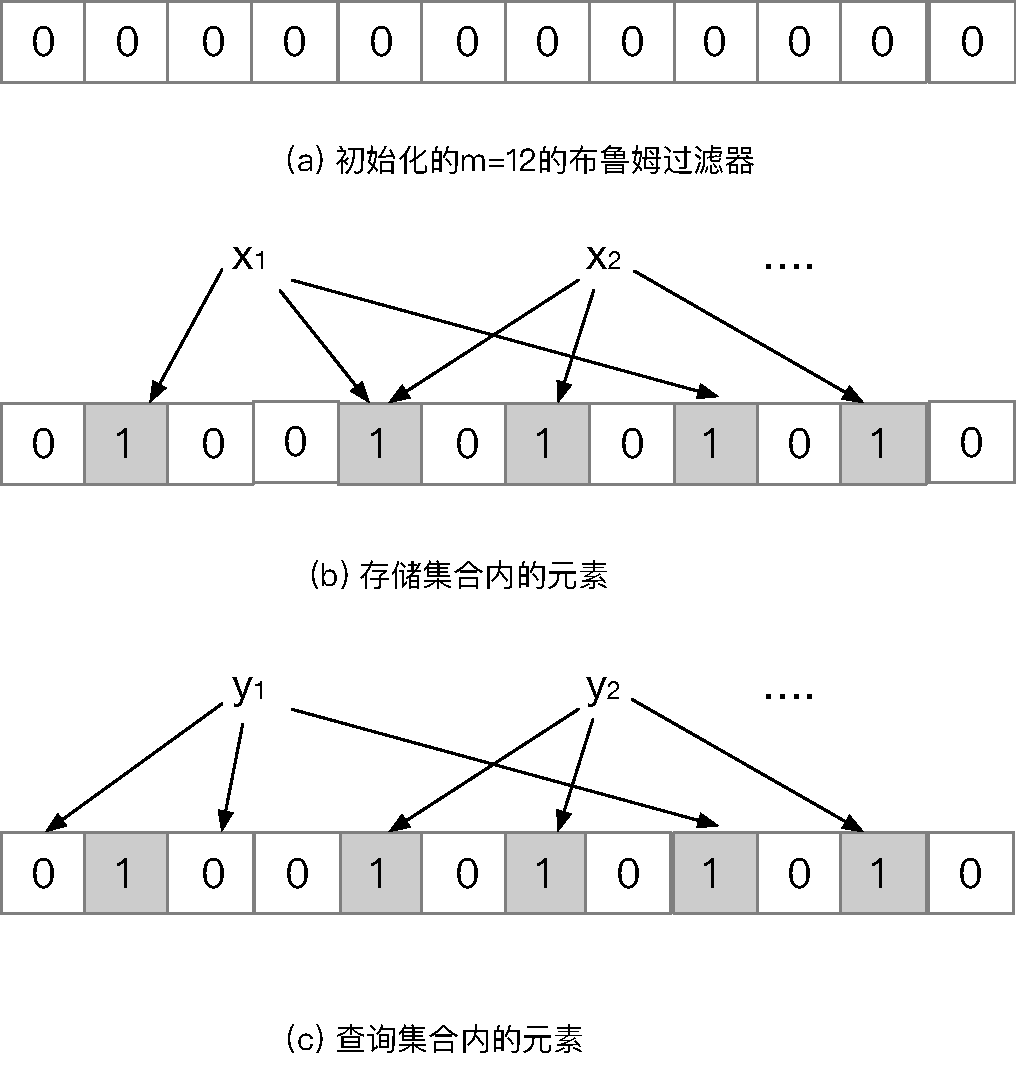
\includegraphics[width=0.65\textwidth]{bloomfilter}
\caption{布隆过滤器}\label{fig:bf}
\end{figure}

换句话说,如果布隆过滤器判断一个元素不在集合中,那肯定就不存在;而如果判断存在,则不一定存在。
下文将对这种不一定存在的原因进行说明。
这种不能确定元素一定存在的问题是由哈希函数可能发生碰撞的特性所决定的。
由此可见,布隆过滤器的高效是以一定的误报为代价的,它通过容忍一定的错误发生的概率换取存储空间的极大节省。
布隆过滤器不适合那些“零错误”的应用场合。

标准的布隆过滤器不支持删除操作。
考虑在图~\ref{fig:bf}(b)中删除元素x$_2$,意味着将位数组内的第5、7、11位置0,此时如果查询元素x$_1$时会得到该元素不存在的结果,因为它对应的第5位上的值在删除x$_2$时被置0了。

标准布隆过滤器的实现中有几个重要参数:误判率\begin{math}\epsilon\end{math}、负载因子\begin{math}\alpha\end{math}、哈希函数的个数k、位数组大小m和集合中元素的个数n。
误判率可通过调整位数组大小或者哈希函数个数进行控制。
下面将对这些参数进行分析,以确定实现标准布隆过滤器的最佳参数组合。

\subsection{误判率估计}
在进行正式的误判率估计前先明确几个定义:
\begin{definition}
	假阳性(false positives)也叫误判,是指当前元素不在集合内,但由于哈希冲突的缘故存在其它元素被映射到部分相同bit位上,从而有一定的概率导致在判定该元素时认定其对应的所有位置都为1,从而判定其在集合内,造成一次误判。这个概率本文称为误判率,误判率用$\epsilon$表示。
\end{definition}

\begin{definition}
	假阴性(false negatives),也叫漏报,是指在位数组内删除某个元素时,导致其他元素对应的比特位被置0,造成本来存在的元素被漏报成不存在。
\end{definition}

\begin{definition}
	负载因子是指集合中存储的元素的个数\textit{n}和布隆过滤器位数组的长度\textit{m}之间的比值,它用$ \alpha $表示,其中$ \alpha  = {n/m} $。
  当$\alpha $为0时,表示布隆过滤器为空,$ \alpha $为1表示布隆过滤器满载。
\end{definition}

下面进行误判率$\epsilon$的计算公式的推导。
首先假设布隆过滤器中使用的k个哈希函数的计算结果都是均匀分布的,即每个元素都等概率地被哈希到m个bit位上的任何一个,与其他元素被哈希到的位置无关。
则对某一特定bit位在一个元素由特定哈希函数插入时没有被置位为1的概率p$_1$为:
\begin{equation}
p_1 = 1-{1/m}
\end{equation}
则k个哈希函数中都没有一个对其置位的概率p$_2$:
\begin{equation}
p_2 = {p_1}^k
\end{equation}
如果插入n($n\leqslant m$)个元素,但都未对其置位的概率p$_3$:
\begin{equation}
p_3 = {p_2}^n = {p_1}^{kn}
\end{equation}
则此位被置位的概率p$_4$为:
\begin{equation}
p_4 = 1 - \left(1 - {1/m}\right)^{kn}
\label{equ:alpha}
\end{equation}
在进行元素查询时,如果待查询元素对应的k个位全部置位为1,则可判定其在集合中。因此将某元素误判的概率为:
\begin{equation}
\epsilon = \left(1 - \left(1 - {1/m}\right)^{kn}\right)^k
\label{equ:epsilon}
\end{equation}


由
$ \left(1 + x\right)^{{1/x}} \thickapprox e $
可知,当m很大时,满足
$-{1/m}$ $\to 0$,
可将公式\ref{equ:epsilon}转化为:
\begin{equation}
\epsilon = \left(1 - \left(1 - {1/m}\right)^{{-m}\frac{-kn}{m}}\right)^k \thickapprox \left(1 - e^{-\frac{nk}{m}}\right)^k
\label{equ:beta}
\end{equation}
由公式\ref{equ:beta}可以初步断定$\epsilon$由元素的个数n和位数组的长度m决定,增大n或者减小m都会导致$\epsilon$的升高。
$m$和$n$的比值就是布隆过滤器的空间开销。
这种计算方法不严格,因为前面假设哈希函数和散列后值的分布是相互独立的。
但是,这个假设随着m和n的增大误判率更接近真实的误判率。
Mitzenmacher证明无假设情况下的误判率的期望值相同\cite{mitzenmacher2002compressed}。

\subsection{最优哈希函数个数}
\label{sec:num_hashf}
哈希函数的选择对于布隆过滤器的性能以及空间利用率都有至关重要的作用。
对于选取什么样的哈希函数已经在前文中有过介绍,这里不再赘述。
而对于哈希函数的个数,直观的认为越多越好。
实际上,哈希函数越多,用于表达集合中每一个元素所需要的位数就越多,这与布隆过滤器用较低的误判率换取空间的高效利用的初衷相悖。那么哈希函数的个数k应该满足什么条件才能发挥最佳性能呢?

下面推导对给定的$\alpha$,k满足什么条件可以使$\epsilon$最小化。

令:
\begin{equation}
f\left(k\right) = \left(1 - e^{-{nk/m}}\right)^k 
\end{equation}

取 b = e$^{n/m}$,得:
\begin{equation}
f\left(k\right) = \left(1 - b^{-k}\right)^k 
\end{equation}

两边取对数得: 
\begin{equation}
lnf\left(k\right) = kln\left(1 - b^{-k}\right)
\end{equation}

函数两边对k求导得:
\begin{equation}
{1/f(k)}\cdot f'(k) = ln(1 - b^{-k}) + k \frac{b^{-k}\cdot lnb}{1 - b^{-k}} 
\label{equ:fk}
\end{equation}

对式~\ref{equ:fk}右边求最值。

令:
\begin{equation}
\begin{split}
\frac{1}{f(k)}\cdot f'(k) = ln(1 - b^{-k}) + k\cdot \frac{b^{-k}\cdot lnb}{1 - b^{-k}} = 0 \\
\Rightarrow (1 - b^{-k}) ln(1 - b^{-k}) = -k\cdot b^{-k}\cdot lnb \\
\Rightarrow 1 - b^{-k} = b^{-k} \\
\Rightarrow e^{-\frac{kn}{m}} = \frac{1}{2}\\
\Rightarrow k = ln2\cdot {m/n} \thickapprox 0.7{m/n}
\end{split}
\end{equation}
因此,对于固定的$\alpha$,当$k = 0.7{m/n}$时具有最低的误判率,此时$\epsilon$等于:
\begin{equation}
(1 - {1/2})^k = 2^{-ln2\cdot\frac{m}{n}} \thickapprox 0.62{m/n}
\end{equation}

\subsection{最优位数组长度}
\label{sec:opt_m}
对于给定的误判率上限,布隆过滤器至少需要多少位才能表示全集中任意的x个元素的集合?
假设全集中元素的个数为n,最大误判率为$\epsilon$。以此为前提展开对位数组大小应满足的条件进行分析。

假设$S_n$为全集中任取$n$个元素的集合,$B$是用于表示$S_n$的位数组。
那么对于集合$S_n$中任意一个元素$x$,在$B$中查询$x$都能得到肯定的结果,即$B$能够接受$x$。
显然,由于布隆过滤器允许一定的误判率,$B$能够接受的不仅仅是$S_n$中的元素,它还允许最多$\epsilon \cdot(u - n)$个误判。
因此,对于一个确定的位数组来说,它能够接受总共$n +\epsilon\cdot(u - n)$个元素。
在$n + \epsilon\cdot(u - n)$个元素中,$B$真正表示的只有其中$n$个,所以一个确定的位数组可以表示:
\begin{equation}
\binom{n + \epsilon \cdot(u - n)}{n}
\end{equation}
个集合。
$m$位的位数组一共有$2^m$个不同的组合,可以进一步推导$m$位的位数组可以表示:
\begin{equation}
2^m\binom{n + \epsilon *\left(u - n\right)}{n}
\end{equation}
个集合。全集中包含n个元素的子集总共有:
\begin{equation}
\binom{u}{n}
\end{equation}
个。因此,要让布隆过滤器的位数组大小能够满足所有包含n个元素的子集,必须满足:
\begin{equation}
2^m\cdot\binom{n + \epsilon \cdot(u - n)}{n} \geq \binom{u}{n}
\end{equation}
即m需要满足:
\begin{equation}
m \geq log_2({\binom{u}{n}/\binom{n + \epsilon \cdot(u - n)}{n}}) \geq log_2({\binom{u}{n}/\binom{\epsilon u}{n}}) \thickapprox log_2\epsilon^{-n} = n log_2({1/\epsilon})
\label{equ:bfm}
\end{equation}
式~\ref{equ:bfm}中近似相等有个重要的前提条件:$n$远小于$\epsilon\cdot u$,这个前提在处理实际问题中通常是容易被满足的。
根据式~\ref{equ:bfm}中的不等式,得到如下结论:在误判率上限为$\epsilon$的情况下,$m$至少要等于$nlog_2{1/\epsilon}$才能表示任意$n$个元素的集合。

在本章~\ref{sec:num_hashf}中推导出哈希函数的个数$k$等于$k = 0.7{m/n}$时可以得到最小误判率,此时的误判率为$(\frac{1}{2})^{0.7{m/n}}$。
令$(\frac{1}{2})^{0.7{m/n}} \leq \epsilon $,可以进一步推导:
\begin{equation}
m \geq n\frac{log_2({1/\epsilon})}{ln2} = nlog_2e\ast log_2({1/\epsilon}) \thickapprox 1.44n\cdot log_2({1/\epsilon})
\label{equ:bfm2}
\end{equation}

式~\ref{equ:bfm2}说明当k取到最优值时,要保证误判率不超过$\epsilon$,$m$至少要取到最小值的1.44倍。
可以验证,当给定$\epsilon = 0.01$时,存储每个元素需要9.6比特。
而$\epsilon = 0.001 $时,每个元素需要额外的增加4.8比特。
所以,在实际的应用中,对于误判的容忍度不同,要求误判率越低,则存储每个元素需要的比特位越多,相同位数组长度能存储的元素个数就越少。

\section{Cuckoo过滤器的设计}
\label{sec:cbf_para}
传统的布隆过滤器的空间效率高,对插入和查询元素的处理也相当快。
但是它仍然有不足之处——不支持元素的删除操作。
除非能实现没有碰撞的哈希函数,否则布隆过滤器对元素是否存在的误判难以避免。
研究人员能做的就是尽量选择均匀的哈希函数,并且借助一些数据结构的特性有效地对碰撞进行处理。
在上一节介绍了误判率每缩小到原来的十分之一,至少要增加4.8个比特位用于表示一个元素。
另外,现有的实现布隆过滤器元素删除操作的方法使用计数器等方法,将每个比特位都扩张成一个计数值,删除元素时,将对应位置的计数值减1,这种方法增加了空间开销。
所以,布隆过滤器实现更低的误判率和实现删除操作都需要牺牲一定的空间效率。

为了解决上述问题,Bin Fan等人利用Cuckoo哈希方法的特性实现了Cuckoo过滤器\cite{fan2014cuckoo}。
它实现了在布隆过滤器内动态的插入和删除元素,而不会造成漏报。
为了实现动态的插入和删除元素,Cuckoo过滤器采用的是一种称为\textbf{不完整键值(partial-key)} Cuckoo哈希的技术。
Cuckoo过滤器是标准Cuckoo哈希表在集合元素查询算法领域的应用。

\subsection{Cuckoo过滤器的数据结构}

Cuckoo过滤器在基本数据结构上与Cuckoo哈希表类似,因此在介绍Cuckoo过滤器的构造过程之前,先简单回顾一下Cuckoo哈希表的构造过程。
Cuckoo哈希设置了两个哈希函数,分别记作$h_1(x)$和$h_2(x)$,在插入元素时,每个元素有两个备选的哈希桶。
在进行元素查询操作时,检查对应的两个哈希桶内是否存储有该元素。
图~\ref{fig:cuckoo_basic}(a)所示为在一个含有8个哈希桶的Cuckoo哈希表内插入新元素$x$的过程,通过哈希函数计算之后,元素$x$可以被存储到编号为2或者6的哈希桶内。
如果元素$x$对应的两个哈希桶都有空闲位置,则随机选取一个位置将$x$插入,然后结束该次插入操作。
如果两个对应的哈希桶都已经饱和,则将按照图~\ref{fig:cuckoo_basic}(a)所示的过程选择一个备选哈希桶(如编号为6的哈希桶),然后将该哈希桶内的元素(对应元素$a$)踢出,将$a$移动到$h_1(a)$或$h_2(a)$对应的哈希桶内(如果$a$当前存储的桶编号为$h_1(a)$,则$a$将移动到桶编号为$h_2(a)$的哈希桶内,反之亦然。本例中是从编号为6的哈希桶移动到编号为4的哈希桶),若编号为4的哈希桶也没有空闲位置,则继续将元素$c$移动到它对应的另一个备选哈希桶内(过程与移动元素$a$一样)。
一直重复上述过程,直到所有的元素都找到合适的存储位置,或者进行元素移动的次数达到了预先设定的上限值为止(一般地上限值设置为500)。
插入元素$x$之后,Cuckoo哈希表如图~\ref{fig:cuckoo_basic}(b)所示。
如果在某次插入元素时,经过了500次的元素移动仍然有元素没有找到合适的存储位置,则判定哈希表饱和。

\begin{figure}[htbp]
\centering
%\subfigure[Intel]{
\subfigure[插入x之前的哈希表]{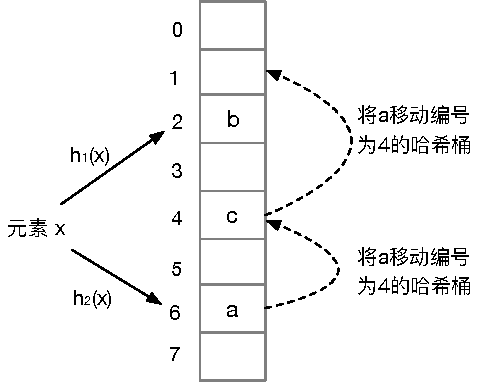
\includegraphics[width=0.45\textwidth]{cuckoo_basic_a}}
\subfigure[插入x之后的哈希表]{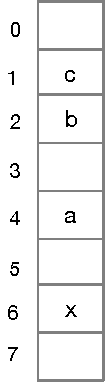
\includegraphics[width=0.1\textwidth]{cuckoo_basic_b}}
\caption{Cuckoo哈希表元素插入过程}
\label{fig:cuckoo_basic}
\end{figure}

Cuckoo过滤器构造过程与Cuckoo哈希表类似:首先创建一个空的Cuckoo哈希表;然后将集合内的元素插入到哈希表内。
% 不同的是在哈希桶内存储的不是完整的元素的键值,而是将元素进行哈希运算成固定大小的\textbf{指纹}(fingerprint)~\cite{memc3}。
% 指纹信息的长度用$f$表示。
如图~\ref{fig:bf}所示,标准的布隆过滤器是一个大数组,它表示元素时需要使用$k$个哈希函数将元素映射到过滤器的$k$
个位置上,对相应的位置置1;判定元素是否存在时,也是通过使用$k$个哈希函数分别进行运算得到$k$个索引值,然后判断对应的$k$个位置是否全为1。
而Cuckoo过滤器很好的利用了哈希表的特性,只需使用一个哈希函数将元素表示成一个固定长度的哈希值,然后按照哈希表插入元素的方法插入即可。
这个固定长度的哈希值在Cuckoo过滤器中被称为指纹,指纹的长度用$f$表示。
其插入元素的过程与标准的Cuckoo哈希表类似,区别在于元素以指纹的形式存储。
元素以指纹信息的形式存储在过滤器内,有利于提高空间利用率,但是同时也会产生一个问题:如果发生如图~\ref{fig:cuckoo_basic}(a)所示的现象,需要为新插入的元素腾出空间而移动旧元素时,无法根据旧元素的指纹信息得到它的备选哈希桶的偏移地址。
解决这个问题的方法使用的是一种称之为不完整键Cuckoo哈希(partial-key cuckoo hashing)的方法,关于该方法的详细介绍在~\ref{sec:insert}小节中给出。
值得说明的是,计算元素指纹信息所用的哈希函数$f(x)$与计算元素哈希桶索引值所用的两个哈希函数是不相同的。
构造Cuckoo过滤器的过程如图~\ref{fig:cf_construct}所示。
为了提高空间利用率和元素查询的速度,Cuckoo过滤器采用(2,4)组相连结构,即使用两个哈希函数,每个哈希桶能容纳四个元素。


\begin{figure}[htbp]
\centering
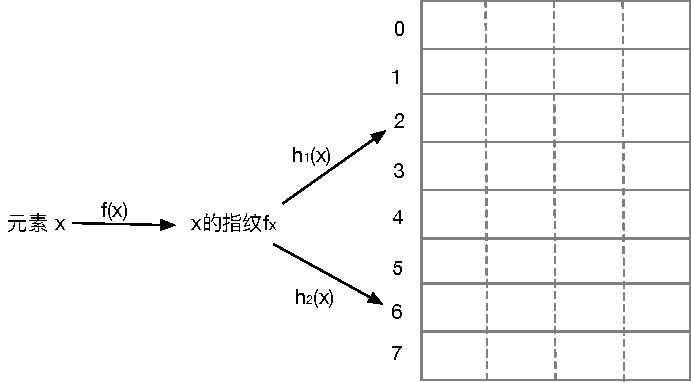
\includegraphics[width=0.8\textwidth]{cuckoo_basic(c)}
\caption{(2,4)组相联Cuckoo过滤器}\label{fig:cf_construct}
\end{figure}

\subsection{Cuckoo过滤器的参数}
这部分重点对Cuckoo过滤器有重大影响的几个参数的理论计算过程进行分析。
方便起见,表~\ref{tab:ckf_para}列出了本小节所用到的一些关键参数及其代表的含义。
\begin{table}[htbp]
  \centering
  \caption{相关符号及其含义}
  \label{tab:ckf_para}
  \begin{tabular}{ll}
    \toprule
      参数  & 含义  \\
    \midrule
      $\epsilon$              &   误判率 \\
        f                 &   指纹信息的长度(单位:bit)\\
      $\alpha$                &   负载因子($0\leq\alpha\leq 1$) \\
      b                             &   每个哈希桶内包含的实体的数量 \\
      m                 &   哈希桶的数量 \\
      n                             &   元素的数量 \\
        C                 &   表达一个元素所需的平均位数(单位:bit)\\
    \bottomrule
  \end{tabular}
\end{table}

\subsubsection{指纹信息的长度}
这部分将通过理论分析指出,使用不完整键Cuckoo哈希方法将元素以指纹的形式存储在Cuckoo过滤器内的方法会导致指纹信息的长度下界值会随着过滤器的规模增加而缓慢增长。
这一点与标准的布隆过滤器不同,标准布隆过滤器每个元素使用多少位进行表示(k值的设定)只取决于预定的误判率。
直观的看,这似乎是Cuckoo过滤器的劣势,但是实验结果表明,这一点对Cuckoo过滤器性能的影响微乎其微。
实验结果表明,当每个哈希桶能够存储4条长度大于等于6 bits的指纹信息时,存储40亿个元素的哈希表的空间占用率达到95\%以上。

\textbf{最小指纹信息长度:}在Cuckoo过滤器中,对于一个给定的元素,根据其当前位置和指纹信息使用不完整键哈希方法可以计算出它的备选哈希桶的索引值。
这样,每个元素的候选哈希桶都不是独立的。
比如,某一元素可以存放在桶$i_1$或$i_2$中,对于长度为$f$比特的指纹信息,根据公式~\ref{equ:ckf},$i_2$可能的索引值最多有$2^f$种可能。
若指纹信息的长度为一个字节,对给定的$i_1$,$i_2$最多只能偏离$i_1$ 256个位置。
对于具有$m$个桶的哈希表而言,当$2^f \leq m$时,$i_2$能够选择的哈希桶的范围只是整个$m$个哈希桶的一个很小的子集。

直观上看如果指纹信息的长度足够长,不完整Cuckoo哈希仍然能够接近标准Cuckoo哈希的冲突处理能力。
然而,如果哈希表非常大,而此时指纹信息的长度相对来说要远远小于哈希表的大小,这样容易引起更多的哈希碰撞,从而导致元素插入失败的概率升高。
当Cuckoo过滤器需要处理大量元素,而$\epsilon$设定一个中等偏低的值时,可能发生上述情形。
接下来,将通过分析确定插入失败的概率下限。

首先分析对于给定的$u$个元素,它们恰好映射到相同的两个哈希桶内的概率$p_1$。
假设第一个元素$x$位于桶$i_1$内,并且指纹为$t_x$。
如果其他的$u-1$个元素具有与$x$相同的桶索引值,它们必然满足以下两个条件:(1)它们的指纹都为$t_x$,出现的概率为$\frac{1}{2^f}$;
(2)它们第一个桶索引值为$i_1$或者$i_1 \bigoplus h(t_x)$,出现的概率为$\frac{2}{m}$。
因此,$u$个元素映射到相同的两个桶内的概率$p_1 = (\frac{2}{m}\ast \frac{1}{2^f})^{u-1}$

现在考虑构建Cuckoo过滤器的随机插入$n$个元素的构建过程。
假设初始化的哈希表桶数组满足$m = cn$,每个哈希桶容纳的元素个数为$b$,其中$c$为常数。
当出现$u = 2b+1$个元素被映射到相同的两个桶内时,表明插入失败。
出现这种情形的概率为插入失败的概率下界。
由于从$n$个元素中包含$2b+1$个元素的子集有$\binom{n}{2b+1}$个,$2b+1$个元素在插入过程中发生碰撞的期望值为:
\begin{equation}
\binom{n}{2b+1}(\frac{2}{2^fm})^{2b} = \binom{n}{2b+1}(\frac{2}{2^f{cn}})^{2b} = \Omega(\frac{n}{4^{bf}}) 
\label{equ:cbf_f}
\end{equation}

因此,由式~\ref{equ:cbf_f}可以做出结论,$4^{bf}$必须满足$\Omega(n)$才能避免异常的插入失败的概率。
指纹信息的长度最好为$f = \Omega(log(\frac{n}{b}))$比特。
在第~\ref{sec:opt_m}节中指出标准的布隆过滤器用于表示每个元素所需的比特数为常数(近似等于$ln(\frac{1}{\epsilon})$)。
而Cuckoo过滤器指纹信息所需的长度为$\Omega(logn)$这个级别,这个结果看上去似乎不是特别理想。
这会不会引起扩展性问题呢?
实验表明桶容量$b$在下界约束中的起决定作用:只要将$b$控制在合理的大小,指纹信息的长度仍然可以保持较小的值。

\textbf{实验评估:}
%实验评估
图~\ref{fig:cbf_fingerprint_size}所示为负载因子$\alpha$与指纹信息长度$f$,哈希桶容量$b$以及哈希表总的哈希桶数量$m$的数量关系曲线。
$x$轴表示指纹信息的长度($1~\leq ~f~\leq ~20$),$y$轴表示负载因子($0~\leq ~\alpha ~\leq 1$)。
图~\ref{fig:cbf_fingerprint_size}(a)、(b)所示分别为$b = 4,8$时指纹信息长度与负载因子的变化关系。
实验时,插入的元素为64位的随机值。
认定哈希表“饱和”的条件是:当执行某次插入操作时,进行了多达500次的替换操作之后仍没有找到空闲的位置接纳被踢出的元素。
当哈希表达到”饱和“之后,停止本次测试并记录此时哈希表的负载因子。
每组参数运行十次,最终结果取十次的平均值。
\begin{figure}[htbp]
\centering
\subfigure[$b$~= ~4 ]{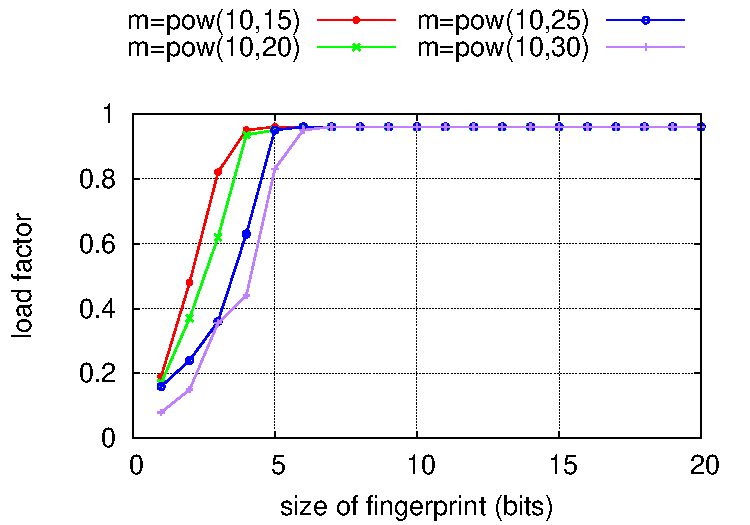
\includegraphics[width=0.45\textwidth]{cbf_loadfactor_b4}}
\subfigure[$b$~ = ~8]{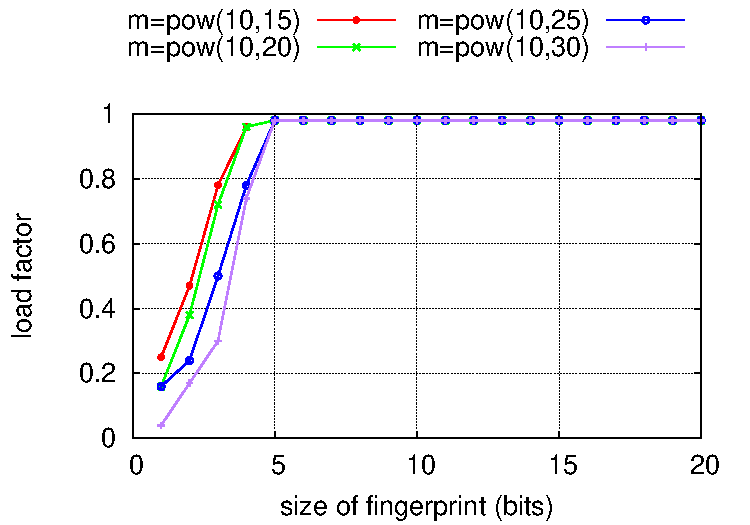
\includegraphics[width=0.45\textwidth]{cbf_loadfactor_b8}}
\caption{负载因子与指纹信息长度变化关系}
\label{fig:cbf_fingerprint_size}
\end{figure}

如图~\ref{fig:cbf_fingerprint_size}所示,在所有的参数组合中,$b = 4$的过滤器的哈希表的利用率能够达到95\%,而$b = 8$的过滤器在指纹信息大小足够长的前提下哈希表利用率可以达到98\%。利用率达到这些值后,增加指纹信息的长度对哈希表利用率的提升几乎没有帮助(但是可以降低误判率)。
通过前文的理论分析表明,当过滤器的规模增大时,所需的$f$的最小值会发生变化。
此外,通过比较图~\ref{fig:cbf_fingerprint_size}(a)和图~\ref{fig:cbf_fingerprint_size}(b)发现达到高哈希表利用率的$f$的最小值随着哈希桶容量$b$的增加而减小,这个规律同样也与前文的理论分析的结果吻合。
在本次实验中,使用两个完全独立的哈希函数,当$b = 4$且$m = 2^{30}$时,哈希表最多能存储多达40亿个元素,而当指纹信息的长度大于6比特时,$\alpha$接近"最优负载因子"。

\textbf{启示:}
通过结合公式~\ref{equ:cbf_f}对$f$的下界约束推导的结果与图~\ref{fig:cbf_fingerprint_size}中的实验结果可以总结出Cuckoo过滤器的一条非常重要的结论。
在理论上Cuckoo过滤器的空间效率要比标准布隆过滤器“差”——
$\Omega(log~n)$与常数的区别。
对于布隆过滤器而言,不论哈希表存储的元素个数是一千、一百万还是数十亿,达到百分之一的误判率大约都只需要10个比特位来表示每个元素。
而为了保持相同的空间效率Cuckoo过滤器需要使用更多的比特位表示每条指纹信息。
同样的由理论推算过程可知,$f$为$\Omega(log~n)$比特,如果$b$足够大,则$f$的值增长非常缓慢,在实际的应用中,可以将其视为常数。
图~\ref{fig:cbf_fingerprint_size}的结果表明6比特的指纹信息足够存储数十亿个元素,并且能够达到很高的哈希表利用率。

\subsubsection{空间效率}
\label{sec:space_ef}
对Cuckoo过滤器内的元素进行增、删、查操作与每个哈希桶内包含多少实体无关。
但是,为Cuckoo过滤器选择正确的参数对于空间效率具有重要意义。
这一部分着重介绍如何选取合适的参数优化Cuckoo过滤器的空间效率。

% \textbf{空间开销:}
空间效率是通过计算在完整的过滤器中用于表示每个元素所用的平均比特数来衡量的。
用哈希表长度(比特)除以过滤器有效存储的元素的个数就是表示每个元素所用的平均比特数。
尽管每个实体可以存储一条指纹信息,但是并不是所有的实体都已经存入了指纹信息——过滤器的哈希表内一定有空闲的实体。
所以,每个元素实际上需要的比特数大于指纹信息的长度。
如果每条指纹信息的长度为$f$比特,哈希表的负载因子为$\alpha$,C的单位为:bits/item,每个元素的空间开销C可以用式~\ref{equ:space_cost}表示。
\begin{equation}
C = \frac{\text{哈希表的比特数}}{\text{存储的元素个数}} = \frac{f\cdot \text{实体的数量}}{\alpha \cdot \text{实体的数量}} = \frac{f}{\alpha} \text{bits.}
\label{equ:space_cost}
\end{equation}

在前文中有过介绍,指纹信息的长度和负载因子都与哈希桶的大小有关。
下面研究在给定的误判率$\epsilon$前提下,如何通过设置哈希桶的容量$b$使$C$达到最小。

保持Cuckoo过滤器的总比特数为常量,调整哈希桶的容量会产生两方面的影响:
\textbf{第一,哈希桶容纳的实体数量越多,哈希表的空间利用率越高。}对于使用两个哈希函数的Cuckoo过滤器,当桶能容纳的实体数$b = 1$时,哈希表的负载因子$\alpha$为50\%,
而当$b = 2,4,8$时,$\alpha$分别为84\%,95\%和98\%。

\textbf{第二,哈希桶的容量越大,维持相同误判率需要的指纹信息的长度越长。}
哈希桶的容量越大,进行查询时需要检查更多的实体,发现相同指纹信息的概率也会增加。
在最坏情况下,查询一个并不存在的元素需要探测两个分别包含了$b$个实体的桶
(当然并不是所有的哈希桶内都填满了实体,这里只是考虑最糟糕的情况;当哈希表的负载因子达到95\%时,已经很接近极限情况)。
对于每一个实体而言,一次查询与存储的指纹相匹配并且返回成功匹配被误判的概率最多为${1/2^f}$。
在进行$2b$次这样的比较之后,误判率的上界为:
\begin{equation}
1 - (1 - {1/2^f})^{2b} \thickapprox {2b/2^f}
\end{equation}
该上界约束与哈希桶的容量$b$成正比。
为了保证预定的误判率$\epsilon$不变,必须确保${2b/2^f}\leq \epsilon$,保证这个条件的最小指纹信息长度为:
\begin{equation}
f \geq \lceil log_2({2b/\epsilon})\rceil = \lceil log_2({1/\epsilon}) + log_2(2b)\rceil  
\label{equ:upper_f}
\end{equation}

由式~\ref{equ:space_cost}和\ref{equ:upper_f}可以推算存储每个元素的空间开销$C$受下面条件的限制:
\begin{equation}
C \geq {\lceil log_2({1/\epsilon}) + log_2(2b)\rceil /\alpha}
\label{equ:space_cost_bound}
\end{equation}
$\alpha$随着$b$的增加而增加。
当$b = 4$时,$\alpha = 0.95$,${1/\alpha} \thickapprox 1.05$。
此时$C$ = 1.05$log_2({1/\epsilon}) + 1.05 * 3$。
式~\ref{equ:space_cost_bound}表明,当负载因子一定时,Cuckoo过滤器的空间开销要低于布隆过滤器($1.44log_2({1/\epsilon})$)。

为了确定最优的哈希桶容量$b$,下面将通过实验比较参数$b$为不同的值时的空间效率。
用不完整键Cuckoo哈希方法构造具有不同的指纹信息长度的哈希表,分别记录对应的平均空间开销和误判率。
结果如图~\ref{fig:cbf_space}所示。
使空间效率最好的$b$的取值依赖于预定的误判率$\epsilon$:当$\epsilon > 0.002 $时,$b = 2$对应的平均空间开销要略好于$b = 4$对应的空间开销;而当$ 10^{-5} < \epsilon \leq 0.002$时,$b = 4$具有最小的空间开销。

\begin{figure}[htbp]
\centering
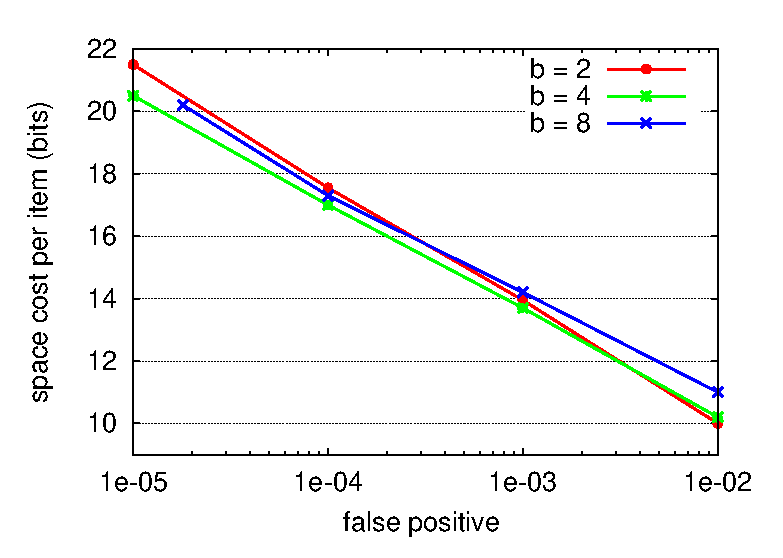
\includegraphics[width=0.6\textwidth]{space.eps}
\caption{哈希桶容量与空间效率的关系}
\label{fig:cbf_space}
\end{figure}

综上所述,Cuckoo过滤器的默认参数配置为(2,4),即每个元素有两个候选的哈希桶,每个哈希桶最多能够容纳4条指纹信息。
选取这组参数作为默认配置的原因有两个方面:一是实际的应用一般都要求误判率满足:$ 10^{-5} < \epsilon \leq 0.002$~\cite{broder2004network};二是这个参数组合能够提供最优综合性能。

\section{并发Cuckoo过滤器}
无论是标准的布隆过滤器还是现有的其他布隆过滤器的扩展版本,都具有在单核平台上快速处理元素的能力以及高效的空间利用率。
单核处理器的计算能力已达到瓶颈,相对而言多核计算机的计算资源和计算能力更加充裕。
在当前数据呈现爆炸式增长的背景下,海量数据处理压力越来越大,基于单核处理器的过滤器逐渐显得捉襟见肘。
因此,设计基于多核系统并发过滤器对于海量数据处理是具有重大实际意义的工作。
然而,当前的相关研究中并没有一款支持并发查询和更新的过滤器。

并发控制机制是在多核平台上设计并发数据结构的关键环节,它对线程扩展性和整体性能起决定作用。
在前面对并发哈希表的评估与分析中通过比较各个并发哈希表的线程同步方式发现,不当使用共享变量以及使用TAS锁不利于并发哈希表的线程扩展性。
本文设计的并发Cuckoo过滤器的基础数据结构本质上仍然是哈希表,不同的是Cuckoo过滤器根据处理集合成员查询问题的特征,改用存储不完整键值替换标准Cuckoo哈希表中存储完整的键值信息的做法,换取存储空间的极大节省。
因此,前文通过实验评估得出的结论仍然适用于并发Cuckoo过滤器。
这一部分主要介绍并发Cuckoo过滤器的实现过程和性能评估结果。

\subsection{自旋锁}
在设计并发数据结构时,如果临界区非常小(比如,只包含几条或者几十条指令),则可以考虑使用时旋锁(spinlock)。
因为使用普通的互斥锁会涉及到操作系统的调度。
自旋锁的工作方式是让竞争的线程不断地读取一个变量(locked)的状态,判断是否满足进入临界区的条件。
在前文的第~\ref{sec:rtm_lock}小节中,介绍了一种名为MCS的自旋锁。
这里再介绍几种常用的自旋锁——TAS锁,TTAS锁和CLH锁,并解释选择MCS锁作为实现并发Cuckoo过滤器的原因。

TAS(test-and-set)锁是一种简单的自旋锁。
其实现代码如算法~\ref{algo:tas-lock}所示。
test\_and\_set()操作用于早期的多处理器架构上解决同步问题,它利用CPU提供的指令(如X86的xchg,LOCK指令前缀等)对内存地址(或者字节)进行操作。
该内存地址上存储的是一个布尔变量,值为$true$或$false$。
TAS指令原子地完成以下操作:
写入true到这个地址,并返回这个地址上存储的旧值。
从表面上看,TAS指令是实现自旋锁的理想选择。
当lock的值为$false$时,表明当前锁处于空闲状态,可以被占有,当值为$true$时,则表明当前锁正在被其它线程占有。
$spin\_lock()$方法不断的重复执行TAS指令,直到返回$false$。
释放锁时,调用$spin\_unlock()$,将$lock$的值设置为$false$。

\SetKwProg{Fn}{Function}{}{}
\begin{algorithm}[htbp]
\Fn{spin\_lock (lock)}{
   \textbf{while}~(test\_and\_set(lock,~true))\;
}
\Fn{spin\_unlock (lock)}{
  atomic\_set(lock, false)\;
}
\caption{TAS锁}
\label{algo:tas-lock}
\end{algorithm}

实际上在SMP系统上,TAS锁的性能不理想。
原因有两个:其一,TAS中,每次执行锁的get\_and\_set()方法,会独占总线以发送锁的状态变量被修改的消息,
导致其它处理器执行get\_and\_set()时都需要等待,出现串行执行。
其二,每一次执行TAS都必须读-写$lock$变量,这涉及到多个CPU之间的缓存一致性问题。比如,当CPU $P_1$读取$lock$时,如果$lock$不在$P_1$的缓存内,则需要从主存中读入。考虑到$P_1$需要修改$lock$,所以将$lock$从主存读入缓存后,需要将其它CPU上缓存的副本失效(Invalidate)。
存在多个CPU竞争同一个TAS锁时,每一次TAS操作都需要完成以上操作,在系统总线上会产生大量的一致性流量。
此外,在释放锁时,由于总线一直被执行test\_and\_set()方法的处理器占用,导致释放锁被延迟。
因此,随着CPU数目的增多,性能衰减得很快。

TTAS(test-and-test-and-set)锁是在TAS锁的基础上进行改进的一种自旋锁。
当线程A持有锁时,TTAS锁算法的行为如下:当线程B第一次读取锁时,发生缓存未命中,强制使线程B在加载变量$lock$到它的缓存时阻塞。
只要A持有锁,B不断的重复读取$lock$变量,总是能在它的缓存中命中。
这样B不会造成任何的总线流量,也不会导致其它线程的内存访问延迟。
% 此外还有效的解决了在释放锁时出现延迟的问题。
算法~\ref{algo:ttas-lock}简单描述了其实现方式。

但是TTAS锁在释放锁时会出现问题:持有锁的线程通过修改$lock$变量的值为$false$释放锁,这会导致正在进行自旋的线程的缓存副本立即失效。
每个在$lock$上自旋的线程都发生一次缓存未命中,重新从主存中读入新的值,然后调用test\_and\_set()方法获取锁。
第一个成功获取锁的线程会使其它线程的缓存行失效,这些线程必须重新读入$lock$变量,这将引起总线上的流量风暴(storm of bus traffic)。

\SetKwProg{Fn}{Function}{}{}
\begin{algorithm}[htbp]
\Fn{spin\_lock (lock)}{
   \While{test\_and\_set(lock,~true)}{
   \textbf{while}~(lock ~!= false)\;}
}
\caption{TTAS锁}
\label{algo:ttas-lock}
\end{algorithm}

CLH(Craig, Landin, and Hagersten locks)\cite{craig1993building, magnusson1994queue}:也是一种自旋锁,与MCS锁一样,都是以其发明人名字的首字母命名,名字本身不涉及它的实现原理。
CLH锁能确保无饥饿性,提供先来先服务的公平性。
它是一种基于链表的可扩展的、高性能、公平的自旋锁,申请线程只在本地变量上自旋,不断轮询前驱的状态,如果发现前驱节点释放了锁,就结束自旋进入临界区。
CLH队列中的节点QNode中含有一个locked字段,该字段若为$true$表示该线程需要获取锁,且不释放锁,为$false$表示线程释放了锁。
结点之间是通过隐形的链表相连,之所以叫隐形的链表是因为这些结点之间没有明显的next指针,而是通过myPred所指向的节点的变化情况来影响myNode的行为。CLH锁上有一个tail指针,始终指向队列的最后一个节点。

当一个线程需要获取锁时,会创建一个新的QNode,将其中的locked设置为true表示需要获取锁,然后线程修改tail指针,使自己插入到队列的尾部,同时获取一个指向其前趋的引用myPred,然后该线程就在前趋结点的locked字段上自旋,直到前趋结点释放锁。
当一个线程需要释放锁时,将当前结点的locked域设置为$false$,同时回收前趋结点。
如图~\ref{fig:clh_lock}所示,线程A需要获取锁,其myNode域为true,此时tail指向线程A的结点,随后线程B插入到线程A后面,tail指向线程B的节点。然后线程A和B都在它的myPred域上旋转,一旦它的myPred结点的locked字段变为false,它就可以获取锁执行。
图中线程A的myPred的locked域为$false$,表明A的前驱节点释放了锁,并且将A的locked域设置为$false$,线程A结束自旋进入临界区。

\begin{figure}[htbp]
\centering
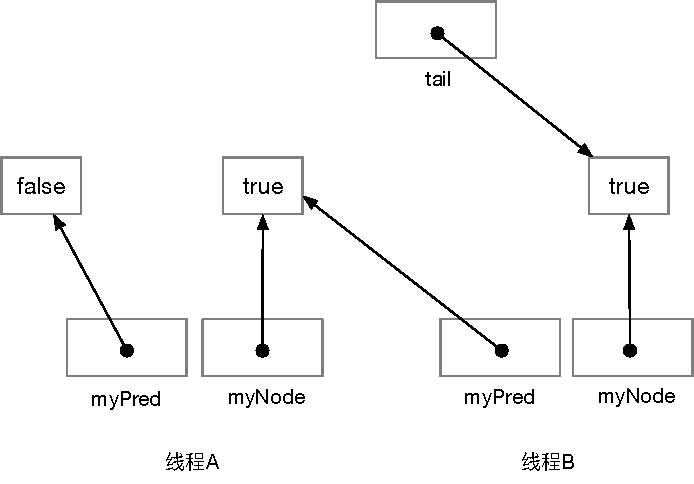
\includegraphics[width=0.8\textwidth]{clh_lock}
\caption{CLH锁结构}
\label{fig:clh_lock}
\end{figure}


CLH队列锁的优点是空间复杂度低(如果有n个线程,L个锁,每个线程每次只获取一个锁,那么需要的存储空间是O(L+n),n个线程有n个myNode,L个锁有L个tail)。
它的缺点是:在NUMA架构下,每个线程都有自己的内存,如果前趋节点的内存位置比较远,自旋判断前趋节点的locked域,性能将大打折扣,但是在SMP系统结构下CLH的性能还是可以保障的。

综合比较上述几种自旋锁的优缺点,在实现并发Cuckoo过滤器时决定采用MCS锁。

\subsection{加锁与解锁}
接下来的内容介绍如何通过基于Intel RTM的MCS锁实现多线程并发的Cuckoo过滤器。
实现Cuckoo过滤器的多线程并发使用的是读写锁,算法~\ref{algo:mcs_lock}给出了基于Intel RTM的MCS锁算法实现。
使用RTM Retry机制来消除TSX Lemming效应对性能的抑制。
其中结构体$spe\_mcs\_lock\_t$是一个对齐的$mcs$锁字段,而结构体$locklib\_mutex\_t$是一个互斥锁字段,它包含了$mcs$锁字段、一个$uint8\_t$类型的$mode$变量以及一个用于缓存行对齐的字符串的结构体。
函数$locklib\_mutex\_lock()$具有两个参数,一个为互斥量$mutex$,一个为整型数$mode$。
$mode$的值分别对应0、1,0表示当前持有锁的线程为读者线程,1表示当前持有锁的线程为写者线程(执行的是删除或插入操作)。
\SetKwProg{Fn}{Function}{}{}
\begin{algorithm}[htbp]
\SetAlgoLined
 \Fn{locklib\_mutex\_lock~(locklib\_mutex\_t ~*mutex, \textbf{uint8\_t} mode)}{
   spec\_mcs\_lock\_t *lock = (spec\_mcs\_lock\_t *) ~mutex; \\
   $reason$ = 0 ;\\
   \textbf{speculative\_path:}\\
   XBEGIN(fallback\_path, reason)\;
   \If{$lock$ is locked} {
       XABORT(1);}
   \KwRet {$0$}\;
   ~~\\
   \textbf{fallback\_path:}
   ~~$retries = retries +1$\;
   \While{$lock$ is locked}{cpu\_relax()\;}
   \If{$retries$ < MAX\_RETRIES}{
     \textbf{goto} speculative\_path\;
   }
  \tcc{以标准方式申请辅助锁}
  my\_node.locked = $true$\;
  qnode\_t = \_\_sync\_lock\_TAS(\&lock->lock, \&my\_node)\;
  \If{$prev$ != NULL}{
    prev->next = \&my\_node\;
    \While{my\_node.locked is $true$}{
      cpu\_relax()\;
    }
  }

  mutex->mode = mode\;
  \KwRet {$0$}\;
 }
\caption{基于Intel RTM的MCS锁算法}
\label{algo:mcs_lock}
\end{algorithm}
对临界区的保护设置了$speculative\_path$,$fallback\_path$两条执行路径:一条为事务化推测执行路径(第16行);一条为回退路径(第21行),即当事务执行失败后,临界区申请标准锁完成本次操作。
在事务化推测执行期间,线程首先不会申请获取锁,直到执行完成准备提交时再申请获取锁,如果申请的锁被占用,则该线程所执行的事务被中止,
线程对系统状态所做的更改都失效,系统回退到初始状态并跳转到回退路径执行(事务内存的原子性)。

跳转到回退路径之后,如果当前重试的次数没有达到预先设定的门限值,将继续尝试进行事务化推测执行(第23-26行)。
如果当前重试次数已经达到了门限值,则使用标准的锁方法完成操作(第29-35行)。

由于硬件事务内存不能保证每次事务化执行都能成功提交对系统状态的更改。
为了避免进程悬停,在使用硬件事务内存进行锁省略编程时设置回退路径是有效的保障程序顺利执行的手段。
一般的,事务代码在经过一定次数的重试之后成功提交的概率远远大于失败的概率,所以执行回退路径对性能的影响是可控的。

\SetKwProg{Fn}{Function}{}{}
\begin{algorithm}[htbp]
\SetAlgoLined
\Fn{locklib\_mutex\_unlock(locklib\_mutex\_t *mutex)}{
          spec\_mcs\_lock\_t *lock = (spec\_mcs\_lock\_t *) mutex\;
          \eIf{XTEST()}{
            XEND()\;
          }{
            \tcc{使用标准的方式进行解锁}\
            qnode\_t *last = my\_node.next\;\
            \If{$last$ == NULL}{
              \If{$true$ == \_\_sync\_bool\_CAS(\&lock->lock, \&my\_node, NULL)}{\KwRet {$0$}\;}
              \While{(last = my\_node.next) == NULL}{
                 cpu\_relax()\;
              }
            }
          my\_node.next = NULL\;
          last->locked = $false$\;
          }
          $retries$ = 0\;
          \KwRet {$0$}\;
}

\caption{基于Intel RTM的MCS解锁算法}
\label{algo:mcs_unlock}
\end{algorithm}

算法~\ref{algo:mcs_unlock}展示了对应的解锁过程。
与加锁过程的两条路径相对应,释放锁的过程也分为两个阶段:首先使用\textit{XTEST}判断当前执行的操作是否为事务执行,若为事务执行,使用\textit{XEND}结束;若判断此次操作申请的锁是通过标准的方式获取的,则按照标准锁的释放过程释放锁。
最后将\textit{retries}变量清零。

\subsection{并发访问接口}

\begin{table}[htbp]
  \caption{HashTable类的成员函数列表}
\label{tab:cbf_API}
\footnotesize
\centering
\begin{tabular}{lll}
\toprule
序号&API &   描述  \\
\midrule
1	&	explicit ~\textbf{HashTable(num)}									 	&  	构造函数\\
2	&	 ~\textbf{HashTable()}  									& 	析构函数\\
3	&	size\_t  \textbf{NumBuckets()} 									&  	返回哈希桶数量\\
4	&	size\_t  \textbf{SizeInBytes() }									&  	返回哈希表大小(单位:Bytes)\\
5	&	size\_t  \textbf{SizeInTags()} 									&  	返回哈希表容纳的指纹的数量\\
6	&	string   \textbf{Info()} 											&  	返回哈希表的容量信息\\
7	&	uint32\_t  \textbf{ReadTags(i, j)}										&  	读取指纹信息\\
8	&	void  \textbf{WriteTags(i, j, t)} 										&  	修改指纹信息\\
9	&	bool  \textbf{ ConFindTagInBuckets(i1, i2, tag) }			& 	并发查找接口\\
10	&	bool  \textbf{ ConDeleteTagFromBucket1(i, tag)	}			& 	并发删除接口\\
11	&	ReturnCode  \textbf{ ConInsertTagToBucket(i, tag, kickout, \&oldtag) }	& 并发插入接口\\
\bottomrule
\end{tabular}
\end{table}

并发Cuckoo过滤器的开发和测试使用C++。
在这一部分中,将对并发Cuckoo过滤器\textbf{HashTable}类的主要API进行介绍。
表~\ref{tab:cbf_API}~列出了Cuckoo过滤器的\textit{HashTable}类的主要API。
序号3-5对应的API主要用于统计哈希表的信息,用于最终计算哈希表的负载因子,内存消耗等;序号6对应的API输出指纹信息的长度、每个哈希桶能容纳的指纹信息的数量、哈希桶的数量、哈希表的最大指纹容量等信息;序号7、8对应的API分别用于读取和修改指定的指纹信息;序号9-11对应的API实现在哈希表内并发的读取和修改元素。

下面对Cuckoo过滤器的三种元素操作的多线程并发实现进行描述。

\subsubsection{插入操作}
\label{sec:insert}
在标准Cuckoo哈希表中,在哈希表中插入新的元素时需要以某种方式读取原本存储于哈希表内的元素,以便在发生踢出原始元素时确定将该元素安置在哪个位置上。
但是,对于只存储了指纹的Cuckoo过滤器而言,它无法根据原始元素的键计算出旧键迁移到哪个位置。
这里引入不完整键Cuckoo哈希算法来解决无法根据指纹信息定位旧键迁移位置的问题。
对任意的元素\textit{x},使用公式~\ref{equ:ckf}计算其两个备选哈希桶的索引值:
\begin{equation}
\begin{split}
h_1\left(x\right) &= hash\left(x\right) \\
% \label{equ:ckf1}
% \end{equation}
% \begin{equation}
h_2(x) &= h_1(x)\bigoplus hash(\text{x的指纹信息})
\end{split}
\label{equ:ckf}
\end{equation}

式~\ref{equ:ckf}的异或操作有一个重要的特性:$h_1(x)$可以通过$h_2(x)$和指纹信息用同样的公式推算出来。
即就是说,替换编号为$i$的哈希桶中的旧键(不论$i$对应的是$h_1$还是$h_2$),都可以通过当前桶编号\textit{i}以及存储在该桶内的指纹直接计算出旧键的备选哈希桶的编号\textit{j},计算方式为:$j = i \bigoplus hash(\text{指纹信息})$。

因此,在进行插入操作时,不用检索目标哈希桶内存储的元素的完整信息,只需要存储在哈希表中的指纹信息。

另外,为了使众元素在哈希表中均匀分布,在与索引值进行异或运算之前,指纹信息已经进行过哈希运算。
当指纹信息远小于哈希表的大小时,如果直接使用索引值与未经哈希的指纹信息进行异或运算来计算接纳被踢出元素的哈希桶的索引值,那么接纳被踢出的元素哈希桶与原来存储该元素的哈希桶在位置上很近,这样会导致插入的元素过于集中,增加Cuckoo路径的长度。
下面的例子有助于理解上述问题。
使用8比特的指纹信息时,接纳从\textit{i}中被踢出的元素的哈希桶的位置距离\textit{i}的最大距离为$2^8 = 256$。
这是因为在进行异或运算时,会选取索引值的低8位进行运算,而高8位保持不变。
对指纹信息进行哈希能够确保这些元素尽量分散在哈希表的不同位置,从而可以避免哈希碰撞,提高哈希表的空间利用率。
\SetKwProg{Fn}{Function}{}{}
\begin{algorithm}[htbp]
\SetAlgoLined
\# define UPDATE\_LOCK ~~~ locklib\_mutex\_lock(mutex, 1)\\
\# define UPDATE\_UNLOCK ~~~ locklib\_mutex\_unlock(mutex)\\
\Fn{Insert(x)}{}{
f = fingerprint(x)\\
i1 = hash(x)\\
i2 = i1~$~~\bigoplus~~$~hash(f) \\
UPDATE\_LOCK \\
\If{\text{桶i1或i2内有空闲实体;}}{
	{将f存入i1或i2;}\\
	UPDATE\_UNLOCK\\
	\Return $true$
	}

\tcc{当前桶内没有空闲位置}
i = rand(i1, i2) \\
\For{$n=0$ \KwTo $MaxNumKicks - 1$}{
	{从bucket[i]中随机的选择一个实体e;}\\
	{将新插入元素的指纹信息与e的指纹信息交换;}\\
	i = i~~$\bigoplus$~~hash(f)\\
	\If{\text{bucket[i]有空闲实体;}}{
		{将f存储到bucket[i];}\\
		UPDATE\_UNLOCK\\
		\Return $true$
	}
}
UPDATE\_UNLOCK\\
\tcc{哈希表饱和}
\Return $false$
}
\caption{Cuckoo过滤器插入操作}
\label{algo:ckf_insert}
\end{algorithm}
算法~\ref{algo:ckf_insert}给出了使用不完整键Cuckoo哈希方法对Cuckoo过滤器动态插入元素的过程。
使用基于Intel RTM的MCS锁对Cuckoo过滤器进行保护。
在事务化推测执行期间,线程并没有真正持有锁,除非它有提交需求。
所以,使用粗粒度锁对整个哈希表进行保护不会影响线程扩展性。
执行插入操作时,首先计算出元素$x$的指纹信息$f$,然后计算$x$的哈希桶索引值$i_1$、$i_2$。
插入具有相同指纹信息的元素在Cuckoo过滤器内是合法的。
然后在索引值$i_1$、$i_2$对应的任意哈希桶内查找是否有空闲位置,若有,则存入;
若两个桶内都没有空闲位置,则在$i_1$、$i_2$中随机的选取一个哈希桶,随机的踢出该桶内的一个元素,然后将新插入的元素存储到空出来的位置。
被踢出的元素将移动到其备选的哈希桶内,如果备选桶内也没有空闲位置,则重复替换过程,一直到所有的元素都找到存储位置或者替换的次数达到上限值为止。
如果替换次数达到上限值,可以认为哈希表已经达到“饱和”,需要考虑重建更大的哈希表。

指纹信息的长度小于$h_1$和$h_2$的长度造成的后果有两个方面:
\textbf{第一},通过公式~\ref{equ:ckf}计算出的($h_1$, $h_2$)的组合的总数会远远小于使用完整的哈希值计算得到的组合的数量,这将导致哈希碰撞更严重;
\textbf{第二},允许插入两个具有相同指纹的元素\textit{x}和\textit{y},在一个哈希桶内可能出现多个相同的指纹信息是合法的。
但是如果相同的指纹的数量超过2b(b为哈希桶的大小)时,存储其指纹信息的哈希桶会过载。
解决哈希桶过载的途径有多种。
\begin{itemize}
	\item 第一,不实现过滤器删除元素操作,这样每条指纹信息都只需要存储一份副本。这是最简单、直观的方法,但这显然与Cuckoo过滤器的设计初衷不符。
	\item 第二,引入适当的空间开销在哈希桶内加入计数器,插入/删除元素时计数器适当的自增/自减。
	\item 第三,将原始的键存储在其他位置(可以是访存速度较慢的外存上),这样可以在插入元素时查看该记录,避免插入重复的元素。
	但是如果哈希桶内已经存在匹配的实体,则插入的速度相对较慢。
\end{itemize}	

\subsubsection{删除操作}
在标准的布隆过滤器中删除元素需要对整个过滤器进行重建,引起惊人的性能开销。
所以标准布隆过滤器不支持删除操作。
而将布隆过滤器的比特位扩展成计数值的方法需要耗费3-4倍的空间开销。
Cuckoo过滤器可以直接从过滤器中移除相关元素的指纹完成删除操作。

安全的删除元素有一个前提条件:被删除的\textit{x}必须是已经插入到了过滤器中的元素。
否则的话,有可能错删过滤器内具有相同指纹信息的其它元素。
这条原则不仅是对Cuckoo过滤器,同样对其他支持删除操作的过滤器也适用。
有关Cuckoo过滤器的删除过程如算法~\ref{algo:ckf_delete}所示。
执行删除操作时,同样要先得到待删除元素的指纹信息,然后通过哈希函数和指纹信息得到存储该元素的哈希桶的索引值。
然后在对应的哈希桶内找到该元素的指纹信息,完成删除操作。

\SetKwProg{Fn}{Function}{}{}
\begin{algorithm}[htbp]
\SetAlgoLined
\# define UPDATE\_LOCK ~~~ locklib\_mutex\_lock(mutex, 1)\\
\# define UPDATE\_UNLOCK ~~~ locklib\_mutex\_unlock(mutex)\\
\Fn{Delete(x)}{}{
	f = fingerprint(x) \\
	i1 = hash(x); \\
	i2 = i1~~$\bigoplus$~~hash(f) \\
	UPDATE\_LOCK\\
	\If{\text{bucket[i1]或bucket[i2]中含有f}}{
		{从当前bucket内删除f的一个副本;}\\
		UPDATE\_UNLOCK\\
		\Return $true$
	}
	UPDATE\_UNLOCK\\
	\Return $false$
}
\caption{Cuckoo过滤器的删除操作}
\label{algo:ckf_delete}
\end{algorithm}

相比当前其它支持删除操作的布隆过滤器的扩展版本,比如\textit{d-left}计数过滤器,熵过滤器的实现,Cuckoo过滤器的删除操作十分简单。
删除元素时,Cuckoo过滤器首先根据索引值在桶内进行查找;如果在任意的桶内有匹配的指纹信息,则删除该桶内的指纹信息的一个副本。

在删除某个元素后,不需要对这个实体进行清理。
这样可以避免在同一个桶内存有两个具有相同指纹信息的元素时的“误删”。
假设元素\textit{x}和\textit{y}都映射到了桶$i_1$内,并且具有相同的指纹信息\textit{f}。
因为$i_2$ = $i_1\bigoplus hash(f)$,所以它们同样能够保存在桶$i_2$内。
在删除\textit{x}时,不用考虑删除的指纹信息的副本是在插入\textit{x}还是\textit{y}是添加的。
删除\textit{x}后,在桶$i_1$、$i_2$中\textit{y}仍然可以被查询到。

值得注意的是,在上面的例子中删除元素\textit{x}之后,过滤器的误判行为仍然存在。
过滤器中的\textit{y}会在查询\textit{x}时发生误判,因为两者具有相同的桶索引值和指纹信息。
误判行为仍然在近似集合元素查询数据结构接受的范围之内,误判率也仍然满足$\epsilon$的上界约束条件。

\subsubsection{查询操作}
\SetKwProg{Fn}{Function}{}{}

\begin{algorithm}[htbp]
\SetAlgoLined
\# define FIND\_LOCK ~~~ locklib\_mutex\_lock(mutex, 0)\\
\# define FIND\_UNLOCK ~~~ locklib\_mutex\_unlock(mutex)\\
\Fn{Lookup(x)}{}{
	f = fingerprint(x) \\
	i1 = hash(x); \\
	i2 = i1~~$\bigoplus$~~hash(f) \\
	FIND\_LOCK\\
	\If{\text{bucket[i1]或bucket[i2]中含有f;}}{
		FIND\_UNLOCK\\
		\Return $true$
	}
	FIND\_UNLOCK\\
	\Return $false$
}
\caption{Cuckoo过滤器查询操作}
\label{algo:ckf_lookup}
\end{algorithm}

Cuckoo过滤器的查询操作相对简单。
算法~\ref{algo:ckf_lookup}对这个过程做了简单描述。
对于给定的元素\textit{x},首先计算其指纹并根据公式~\ref{equ:ckf}计算出它的两个哈希桶的索引值。
然后遍历这些哈希桶:如果在任何一个桶内找到了\textit{x}的指纹,则返回$true$。否则返回$false$。
值得注意的是,只要哈希桶不发生溢出,就能确保不存在任何误判。

\SetKwProg{Fn}{Function}{}{}
\begin{algorithm}[htbp]
\SetAlgoLined
\# define FIND\_lock ~~~ locklib\_mutex\_lock(mutex, 0)\\
\# define FIND\_unlock ~~~ locklib\_mutex\_unlock(mutex)\\
\Fn{ConFindTagInBuckets(\textbf{const} i1, \textbf{const} i2, \textbf{const} tag)}{
\textbf{char} *p1 = bucktets\_[i1].bits\_, *p2 = bucktets\_[i2].bits\_ \\
\textbf{int} v1 = *(*)p1, v2 = *(*)p2 \\
FIND\_LOCK \\
\If{f == 4 ~~ \&\& ~~k == 4}{
	 \textbf{bool} ~ret $\gets$ hasvalue4(v1, tag) || hasvalue4(v2, tag)\\
	 FIND\_UNLOCK \\
	 \textbf{return} $ret$ 
}
\uElseIf{$f == 8 ~~ \&\& ~~k == 4$}
{
	\textbf{bool} ret $\gets$ hasvalue8(v1, tag) || hasvalue8(v2, tag)\\
	FIND\_UNLOCK \\
	\textbf{return} $ret$
}
\uElseIf{$f == 12 ~~ \&\& ~~k == 4$}
{
	\textbf{bool} ret $\gets$ hasvalue12(v1, tag) || hasvalue12(v2, tag)\\
	FIND\_UNLOCK\\
	\textbf{return} $ret$
}
\uElseIf{$f == 16 ~~ \&\& ~~k == 4$}
{
	\textbf{bool} ret $\gets$ hasvalue16(v1, tag) || hasvalue16(v2, tag)\\
	FIND\_UNLOCK\\
	\textbf{return} $ret$
}
\Else{
	  \For{$j=0$ \KwTo $kTagsPerBucket - 1$}{
	  \uIf{(ReadTag(i1, j) == tag) || (ReadTag(i2, j) == tag)}{
	  	FIND\_UNLOCK;\\
	  	\textbf{return} $true$
	  }
	  }
}
FIND\_UNLOCK; \\
\textbf{return} $false$;
}
\caption{Cuckoo过滤器的并发查询过程}
\label{algo:cbf_confind}
\end{algorithm}

\section{性能优化}
% \section{性能评估}
\subsection{空间性能优化}
布隆过滤器因其高效的空间利用率被用于海量数据索引。
因此在设计布隆过滤器时,在寻求使用更少的比特位表示每个元素的同时保持误判率在可承受的范围之内是十分有意义的工作。

如果Cuckoo过滤器不需要实现元素的删除操作,它的空间效率还可以进一步提升。
具体的,对哈希桶容量为4时的Cuckoo过滤器使用一种半排序方法。
之所以称之为半排序是因为这种排序算法只适用于哈希桶容量为4时的Cuckoo过滤器。
使用半排序技术能够为每一个元素的存储节省1比特的空间。
对哈希桶进行半排序是基于一个重要的事实:哈希桶内存储的指纹信息的顺序与Cuckoo过滤器元素查询的结果无关。
在这个前提下,可以首先对哈希桶内的指纹信息进行排序,然后将排序后的指纹信息进行编码压缩。
这个方法与F.Bonomi等人提出的“半排序哈希桶”技术类似~\cite{bonomi2006improved}。

下面举例说明这种半排序压缩方法如何达到节省空间的目的。
假设每个哈希桶的容量$b = 4$并且每条指纹信息的长度$f$为4比特。
则未经压缩的哈希桶的大小为$4*4 = 16$比特。
然而,如果对哈希桶内所有的4比特的指纹信息进行排序之后(没有存储元素的实体视为存储了变量"0"),经过排序之后总共只有3876种可能的组合结果。
再将这3876种可能的桶-值组合存储到一个额外的表内,然后用指向这个表的索引替换掉原始哈希桶,这样原来的哈希桶就只需要使用12比特的索引结构而不是原来的16比特表示,平均每条指纹信息节省1比特的存储空间。

注意到使用这种预先排列出所有可能组合进行查找的方法需要额外的编码/解码表和间接索引。因此,为了保证查询效率,必须保证编码/解码表足够小以便适用高速缓存的容量。
基于上述考虑,半排序方法只适用于哈希桶容量为4的Cuckoo过滤器中。
另外,当指纹信息的长度大于4比特时,只对它的4个比特位进行编码,余下的比特位将直接单独的存储在原来的哈希桶内。

\subsection{并发性能优化}
在访问共享数据时,为了保证程序的一致性,会损耗程序的性能和扩展性。
因此,有效的减少对共享数据的访问有助于提升程序的性能。

事务内存执行事务代码时,为了保证一致性和正确性,需要维护一个读取集(read set)和一个写入集(write set)。
在进行提交时,事务内存必须验证事务的读取集是一个快照,并且需要对照该快照原子地更新写入集\cite{dalessandro2010norec,dice2006transactional}。
事务执行时的读取集和写入集统称为事务的“足迹”(footprint)\cite{avni2014improving}。
对于硬件事务内存,事务的足迹的大小必须小于缓存行的容量。

在软件事务内存中,有一种称为一致性不敏感的编程模型(consistency oblivious programming, COP)~\cite{afek2011towards},即允许符合特定条件的并发代码部分在不进行一致性验证的情况下执行。
COP可以精简事务足迹的大小,从而消除一部分数据冲突和伪中止(spurious abort),有效的提升基于软件事务内存的并发数据结构的性能和扩展性。
但是,使用COP时,必须在涉及对共享数据进行修改的位置添加检查点,用以验证算法在正确的轨道上执行,如果算法执行过程出现异常,则会以更加保守的方式从检查点处重新开始执行,这需要付出更加高昂的一致性开销。
当前支持硬件事务内存的系统,如Intel HasWell和IBM Power HTM,都不允许软件以任何形式访问或者修改事务的读取集。
所以,这种通过设置检查点的方式无法用于支持硬件事务内存的环境中。

受软件事务内存COP编程模型的启发,H.Avni等人\cite{avni2014improving}设计了一种可以用于硬件事务内存的COP模版。
他们的方法可以概括为:使用COP对基于硬件事务内存的并发数据结构进行优化时,可以考虑对事务进行预处理,将其转化成COP事务。
这种针对硬件事务内存的COP编程模型将原始事务分成两部分:一部分为只读前缀,一部分为更新后缀。
前缀执行时不包含任何同步操作,并产生一个可能不一致的输出。
后缀启动包含两个对象的硬件事务:验证前缀生成的是一个可接受的结果,并执行COP事务所需的所有更新操作。

下面结合算法伪代码(算法\ref{algo:cop})说明COP编程模型是如何突破硬件事务内存访问限制,精简事务的读取集和写入集的。
假设函数$\Gamma$(Gamma)是某个数据结构的一个串行化操作(如哈希表的插入、删除、查询)。
为了使$\Gamma$能够适应COP模型,需要先提取$\Gamma$的最长只读前缀到$\Gamma$ReadOnlyPrefix()。
然后$\Gamma$ReadOnlyPrefix()不使用任何同步操作计算得到$\Gamma$Output(第2行)。
由于可能与其它并发操作存在冲突,所以$\Gamma$Output可能是不一致的甚至是错误的。
得到$\Gamma$Output之后,启动事务(第6行),并调用$\Gamma$Verify($Gamma$Output)函数进行验证(第8行)。
如果$\Gamma$Output是不一致的,则调用XABORT中止该事务(第9行)。
如果是一致的,则继续执行$\Gamma$Complete($\Gamma$Output)(第10行)。
$\Gamma$Complete($\Gamma$Output)会执行所有需要执行的更新操作。

在尝试事务提交时(第16行),首先需要检查全局锁是否空闲(第13行)。
如果锁被占有,当前事务被中止,并返回一个特殊编码(第14行)。
在事务启动时可以对锁进行采样,并在锁被其它线程占用的情况下中止事务。
但是,出现这种情况会被判定为进行了一次重试,会导致错误的回退。
所以,通过第19行的代码,可以避免重新计算新的Read Only Prefix(ROP),并且能够避免被判定为一次重试。
从第22行开始处理事务执行失败需要进行重试的情况。
如果事务中止的原因是容量溢出,则不再重试该事务,因为它仍然面临执行失败的结果。
如果事务是被显示的中止的,比如$\Gamma$Verify函数调用了XABORT指令,则必须重新运行$\Gamma$ReadOnlyPrefix()函数重新计算正确的$\Gamma$Output;
否则,事务中止是由冲突引起的,说明$\Gamma$Output的结果是正确的,事务很有可能在经过一次或者几次重试之后成功提交。
如果重试的次数达到上限值,则获取锁,并运行$\Gamma$函数的串行化版本。

 \SetKwProg{Fn}{Function}{}{}
 \begin{algorithm}[htbp]
 \SetAlgoLined
 \SetKwRepeat{Do}{do}{while}%
% % \SetKwFunction{Insert}{Insert}%
$retries \gets 0$\;
 $\Gamma$Output $\gets$ $\Gamma$ReadOnlyPrefix()\;
\While{locked}{await\;}
$status \gets XBEGIN$\;
\eIf{$status == XBEGIN\_STARTED$}{
  \eIf{$\Gamma$Verify($\Gamma$Output) fail}{
  XABORT;~~~~//\text{如果失败,调用XABORT中止事务}\
  }{
  $\Gamma$Complete($\Gamma$Output);~~~~//\text{执行更新操作}\
  }
  \If{locked}{
  XABORT(WAS\_LOCKED)\;
  }
  XEND\;
}{
  \If{is\_explicit(status, WAS\_LOCKED)}{
  \textbf{goto} line 6;~~~~//\text{重用Output}\
  }
  retries++\;
   \If{status $\neq$ XABORT\_CAPACITY}{
  \If{retries < MAX\_RETRIES}{
  \eIf{is\_explicit(status, BAD\_ROP)}{
  \textbf{goto} line 2; ~~~~//\text{重新计算ROP}\
  }{
  \textbf{goto} line 6; ~~~~//\text{重用$\Gamma$Output}\
  }
  }
   }
   lock()\;
$\Gamma$()\;
unlock()\;
}
 \caption{COP模版}
 \label{algo:cop}
 \end{algorithm}

有了COP模版之后,实现Cuckoo过滤器的COP版本,只需要将Cuckoo过滤器的Insert、Delete和Lookup方法(统一用$\Phi$方法描述)转化成对应的$\Phi$ReadOnlyPrefix(),$\Phi$Verify()和$\Phi$Complete()。
算法~\ref{algo:cfinsert}所示为Cuckoo过滤器的Insert方法的COP版本的实现。

\SetKwProg{Fn}{Function}{}{}
\begin{algorithm}[htbp]
\SetAlgoLined
\SetKwRepeat{Do}{do}{while}%
\SetKwFunction{Insert}{Insert}%
\Fn{CF\_Insert(CF *s, K, V)}{
  ~~~retries $\gets$ 0\;
  \textbf{retry:}~\\
  ~~~*index = CFInsertReadOnlyPrefix(t,K)\;
  \textbf{retry\_verify:}\\
  \While{locked}{
  pause();
  }
  status $\gets$ XBEGIN()\;
  \eIf{status == XBEGIN\_STARTED}{
  CFInsertVerify(index, K)\;
  CFInsertComplete(t, K, V, index)\;
  \If{locked}{XABORT(WAS\_LOCKED)\;}
  }{
  \If{is\_explicit(status, WAS\_LOCKED)}{
  \textbf{goto} retry\_verify\;
  }
  \If{retries++ $\leq$ MAX\_RETRIES}{
  \If{is\_explicit(status, BAD\_ROP)}{
  \textbf{goto} retry\;
  }
  \If{can\_retry(status)}{
  \textbf{goto} retry\_verify\;
  }
  }
  }
  //\text{回退路径}\
  lock()\;
  index = CFInsertReadOnlyPrefix(t, K)\;
  CFInsertComplete(t, K, V, index)\;
  unlock()\;
}
\caption{基于COP编程模型的Cuckoo过滤器的Insert方法}
\label{algo:cfinsert}
\end{algorithm}

使用COP编程模型对基于硬件事务内存的并发数据结构的性能提升有一定的帮助,但是这种方法增加了实现的复杂度。

\section{性能评估}
本文在Cuckoo过滤器的基础上\cite{fan2014cuckoo},实现了基于Intel RTM的并发Cuckoo过滤器,并结合一些软件优化方法进行进一步的优化。
下文为了便于进行性能比较和描述,将并发Cuckoo过滤器记作“CCF”。

\subsection{实验配置和性能指标}

\textbf{实验配置:}所有插入过滤器的元素都是预先采用随机数生成器生成的64位的整型数。
由于生成相同数值的概率极低,所以没有对具有相同值的元素进行排查。
每一次对过滤器的操作请求,过滤器首先使用CityHash\cite{cityhash}生成对应元素的64位哈希值。
每一组数据都是运行10次的结果取平均值得到。
所有实验都是在具有两个Intel Xeon Broadwell EP/EN/EX处理器的机器上运行。
该机器总共有32个物理核(64个逻辑核),内存总容量为64 GB。
CPU的时钟频率为2.1 GHz,三级缓存的容量分别为64 KB,256 KB以及40 MB。
该工作站安装的是Ubuntu 16.04 LTS操作系统。

\textbf{性能指标:}为了充分评估CCF的性能、空间效率、误判率以及与CCF并发性相关的线程扩展性、吞吐量,本文确定了以下几个性能指标:
\begin{itemize}
 \item \textit{空间效率:}用于表示一个元素所需的平均比特数,计算方式是过滤器插入的元素的总的比特位数除以过滤器存储的元素数量,用bits/item表示。
 \item \textit{误判率:}在过滤器的负载因子不再变化之后,通过在过滤器内查询不存在的元素,统计返回值为“True”的查询的次数$false\_count$,然后用$false\_count$除以执行的查询的次数,得到误判率;
 \item \textit{构造速率:}往空的过滤器中不断插入元素直到过滤器“饱和”(判断过滤器“饱和”的依据是当执行某次插入操作返回失败)时为止,总的插入元素的个数除以从空到“饱和”花费的时间,单位为million items/sec。
 \item \textit{吞吐量:}平均每秒所能执行的过滤器元素操作的数量;吞吐量跟工作集、过滤器内元素的密度以及线程数量相关。
 \item \textit{线程扩展性:}吞吐量随着线程数量增长的能力,好的扩展性体现在随着参与运算的线程的增加,对应的吞吐量也增加。
% \item \textit{加速比:}在多处理器上,使用$n$个线程的CCF的构造速率和使用单线程的CF的构造速率的比值。
\end{itemize}    

\subsection{空间效率和误判率}
% \textbf{red}{这部分考虑重新设定实验方案进行修正!!}

首先对比CF和CCF的空间效率和误判率。
过滤器的大小设置成192 MB(为$m = 2^{25}$个能存储4个大小为12比特的指纹信息的哈希桶的哈希表的大小)。
对于CCF,执行测试的线程数设置成机器支持的最大线程数(64),每个线程承担的插入任务是均等的,当线程的某次插入操作失败时,该线程的插入任务终止。
当所有的线程完成插入任务或者被终止时,统计插入元素的个数,最终插入元素的个数为各个线程执行的插入次数的总和。
同样CF停止插入元素的条件也是某次插入返回失败。
误判率计算方法是,在过滤器内查询一个确定不存在的元素,如果某次查询操作返回该元素存在,则记录一次误判。
本次实验中,抽样查询次数为一百万次。
最终误判率通过记录的误判数除以总的查询的次数。
表~\ref{tab:cf_space}列出了CF和CCF的相关测试结果。

在指纹信息长度、过滤器容量一定的前提下,CCF的误判率是串行Cuckoo过滤器的一半;
此外,二者最明显的差距体现在构造速率上,CCF的构造速度大约是串行Cuckoo过滤器的十余倍。
但是,CCF的空间利用率较低,约为串行过滤器的50\%。

\begin{table}[htbp]
  \centering
  \caption{Cuckoo过滤器实现并发前后的性能对照表}
  \label{tab:cf_space}
  \begin{tabular}{lllll}
    \toprule
      过滤器类型  & 插入元素个数 & 单个元素占用的比特位数 & $\epsilon$ (\%) &  构造速度  \\
    \midrule
      CF   &  128.07 (M) & 12.58 (bits) &  0.2       &  5.32 (M items/sec)  \\
      CCF  &  66.9 (M)  & 24.07 (bits)  &  0.1       &  658.06 (M items/sec) \\
    \bottomrule
  \end{tabular}
\end{table}

\subsection{扩展性}
这一部分将对CCF的线程扩展性进行评估。

%首先比较不同的锁实现的总和吞吐量,从中选取性能最好的锁方法,然后针对这种方法再进行更细的评估。
首先综合评估了使用不同软件优化方案的RTM版本。
这些软件方法分别是:基于RTM Retry的版本,用“Retry-CCF“标识,其中$retry$的最大次数设置为10(对于$retries$次数的设定将有专门的内容进行说明);基于SLR的版本,用”SLR-CCF“标识;基于SCM的版本,用”SCM-CCF标识“;以及结合了SLR和SCM的版本,用”MIX-CCF“标识。
图~\ref{fig:cf-locks}展示了这四个不同版本的线程扩展性。
图~\ref{fig:cf-locks}(a)对应处理只读数据集的运行结果,图~\ref{fig:cf-locks}(b)对应处理更新占10\%的数据集的运行结果。
过滤器的参数说明:过滤器的哈希桶数量为$2^{24}$个,
数据结构使用(2,4)路组相连的Cuckoo哈希表,即使用2个哈希函数,每个哈希桶能容纳4条指纹信息,因此过滤器的最大指纹信息存储数量为$2^{26}$,指纹信息的长度为12比特,过滤器的负载因子固定为50\%(之所以不设置成更高的参数,是基于数据集中包含一定比例的插入操作),即初始化的过滤器内存储了$2^{25}$个指纹信息。
此时过滤器的大小为96 MB,远大于测试机器的最后一级缓存的容量(40 MB)。

\begin{figure}[htbp]
\centering
%\subfigure[Intel]{
\subfigure[$u$ = 0]{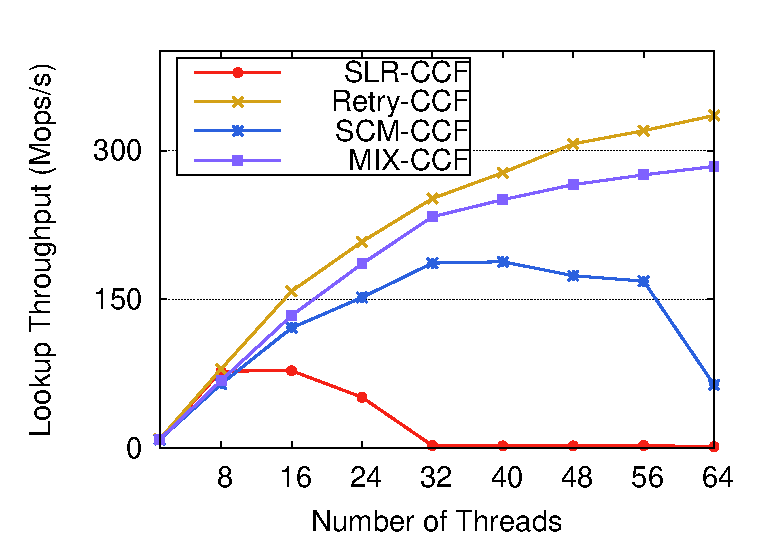
\includegraphics[width=0.45\textwidth]{locks-u0.eps}}
\subfigure[$u$ = 10]{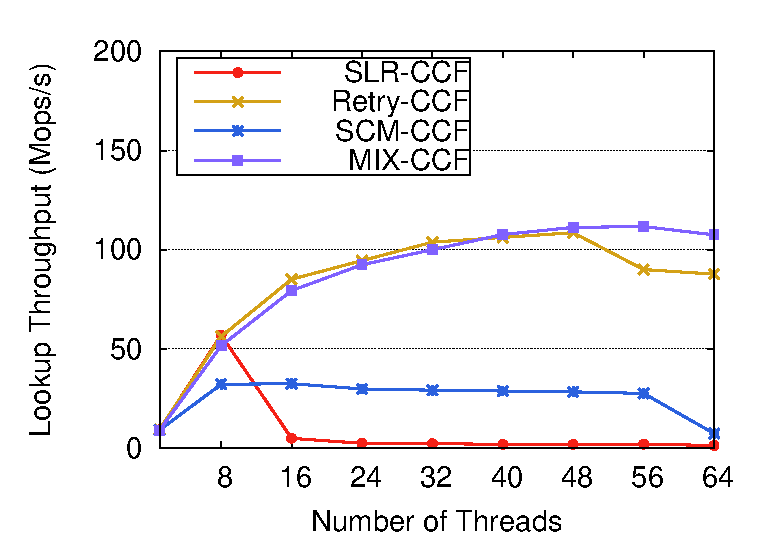
\includegraphics[width=0.45\textwidth]{locks.eps}}
\caption{使用不同软件优化方法的CCF线程扩展性}
\label{fig:cf-locks}
\end{figure}
图~\ref{fig:cf-locks}(a)的结果表明Retry-CCF的扩展性最好,其次是MIX-CCF,单独使用SLR或者SCM的扩展性都不理想;
图~\ref{fig:cf-locks}(b)中Retry-CCF和MIX-CCF的吞吐量和扩展性不相伯仲。
这与第~\ref{sec:htm_global}节中基于HTM的并发哈希表存在差异。

\subsection{更新比重对性能的影响}
Cuckoo过滤器的核心技术是不完整键Cuckoo哈希,是建立在Cuckoo哈希表上的应用。
在对哈希表的综合评估中(第\ref{sec:impact_update})发现数据集中更新比重所占的比例对性能的影响较大。
因此,这里通过几组数据对运行不同数据集的CCF的性能进行比较。
上述对使用不同优化方法的版本进行比较发现基于Retry-CCF机制的性能略胜一筹。
因此,进行这部分测试使用Retry-CCF。
过滤器各项参数的设置与收集图~\ref{fig:cf-locks}数据的设置相同。
不同的是测试所用的数据集包括三个,分别为包含了40\%和10\%更新操作以及只进行查询操作的数据集。
运行的结果如图~\ref{fig:retry_thp}所示。

\begin{figure}[htbp]
\centering
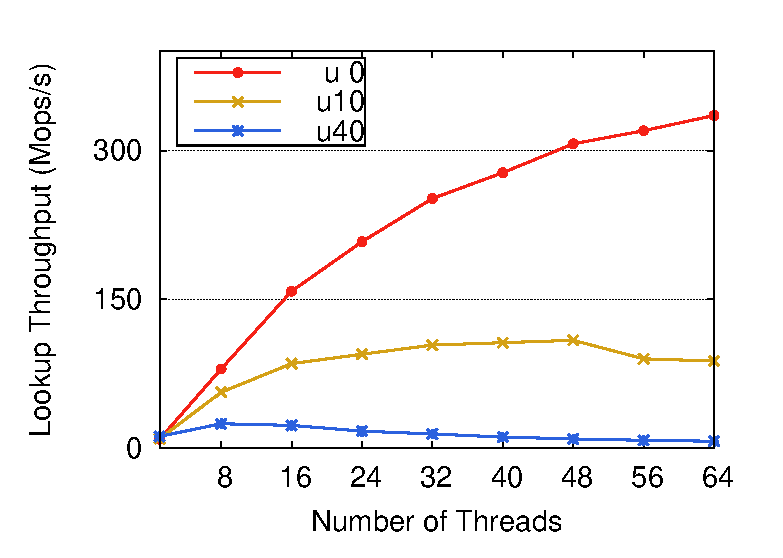
\includegraphics[width=0.65\textwidth]{retries10_throughput.eps}
\caption{并发Cuckoo过滤器的线程扩展性}\label{fig:retry_thp}
\end{figure}

由图~\ref{fig:retry_thp}观察到,并发Cuckoo过滤器的只读性能的扩展性最好,吞吐量随着线程数量的增加而上升,它的最高吞吐量出现在线程数为64处(实验机器支持的最大线程数),是运行单个线程的Cuckoo过滤器的38倍。
而如果测试集中包含一定比例的更新操作时,情况会发生变化。
这种变化直观的体现在吞吐量上,比如数据集包含10\%的更新操作时,最高吞吐量为使用单个线程的11倍,而数据集包含40\%更新操作时,最高吞吐量仅为单个线程的2.5倍。
另外,线程的扩展性也受到数据集中更新操作数量的影响,具体的趋势是数据集的更新操作的比重越高,扩展性就越差。
如在只读的数据集中,一直到线程数达到最大,CCF都展现出良好的扩展性,但在$u = 10\%$时,吞吐量在线程数大于48后出现下降;同样的,$u = 40\%$时,吞吐量在线程数大于16就开始下降。

进一步结合本文第~\ref{sec:thread_scal}中结论,设计或者应用并发哈希表不能一味追求高并发度,要综合考虑工作集的特点。

\subsection{$Retries$设置对性能的影响}
在基于RTM Retry的版本中,$retries$值的设置将直接对性能造成影响。
如果值太小,等待提交的线程在当前持有事务锁的线程释放锁之前就已经转为申请标准锁或者被存放到等待线程队列中,增加了串行化执行的比例,造成性能下降;
如果值过大,某些由系统问题(如页错误、不兼容的指令等)引起的事务中止耗费在Retry过程的时间过长,导致运行效率低。
因此,选用恰当的$retries$值对性能和效率都至关重要。

\begin{figure}[htbp]
\centering
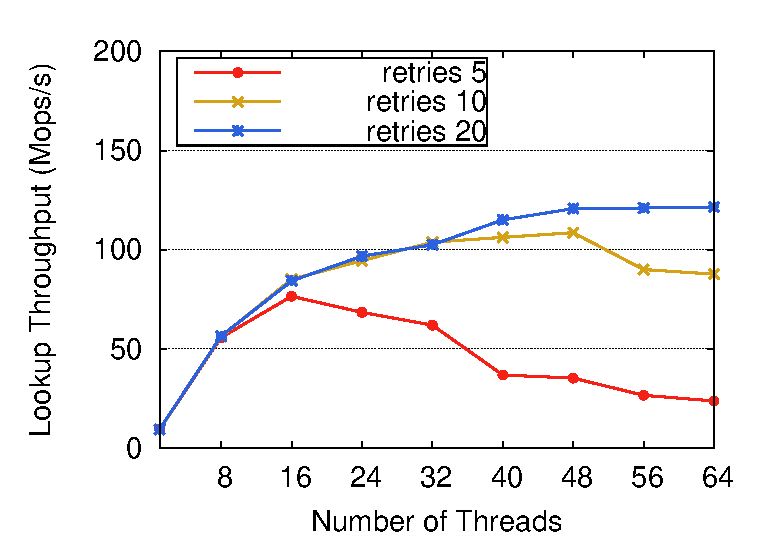
\includegraphics[width=0.65\textwidth]{retries_throughput.eps}
\caption{不同$retries$值之间的性能差异}\label{fig:diff-retry}
\end{figure}

接下来通过一组实验数据说明基于RTM Retry的版本中参数$retries$的设置对并发Cuckoo过滤器性能的影响。
本组实验中测试了$retries = 5, 10, 20$三个值。
测试所用的数据集包含10\%的更新操作。
测试结果如图~\ref{fig:diff-retry}所示。
从图中的曲线趋势可以观察到,当$retries = 5$时,CCF的吞吐量在线程数大于16之后开始下降,并且并发度越高,吞吐量越低。
而$retries$设置成更大的值时,线程扩展性有明显的改善,$retries = 20$的扩展性略微比$retries = 10$的好,但是它所花费的执行时间也更长。
因此,综合考虑扩展性和效率两方面的因素,在本文的相关测试中将$retries$设置为10。

\section{本章小结}
本章首先介绍了标准布隆过滤器的原理,对布隆过滤器的误判率,最优哈希函数个数,位数组长度和空间效率等进行了理论推导。
最终得到位数组长度$m$,元素个数$n$和误判率$\epsilon$之间需要满足:$\frac{m}{n} \geq 1.44 log_2({1/\epsilon})$才能使性能达到最优。
在哈希函数个数一定的情况下,误判率每缩小到原来的十分之一,每个元素平均需要增加4.8比特的存储空间。
随后,介绍了基于不完整键Cuckoo哈希方法的Cuckoo过滤器,对Cuckoo过滤器的设计原理,指纹信息的长度,空间效率,哈希桶的容量等方面都进行了深入的理论分析。
确定了Cuckoo过滤器的空间效率等于指纹信息的长度$f$与过滤器的负载因子$\alpha$的比值。
而$f$与$\alpha$都与哈希桶容量$b$有关,故以此为出发点,进一步的对哈希桶的容量对空间效率的影响进行了分析。
接下来,使用基于Intel RTM实现的读写锁实现了支持多线程并发的Cuckoo过滤器。
对其加锁和解锁算法进行了描述,对并发操作的方法进行详细介绍。
最后对并发Cuckoo过滤器的性能进行了全面的评估。
评估涵盖了对其的线程扩展性、构造速率、误判率、空间效率的评估,评估了与硬件事务内存特性相关的参数的影响以及使用不同软件优化方法对性能的影响。

实验评估的结果表明,我们的并发Cuckoo过滤器在多核处理器上的效率和性能都与预期的结果相符,在处理只读数据集时最高吞吐量是使用单个线程运行的
38倍,数据集中包含少量更新操作时,吞吐量略低,但也达到单个线程处理的吞吐量的11倍。
此外还发现在支持硬件事务内存的环境里使用简单的优化方案带来的性能上的改善效果更明显。






